%!TEX root = practicum2.tex
The performance of the perceptron trained with the Minover algorithm can be measured using the generalization error defined in \autoref{eq:method:generalization_error}. To explore the behaviour of the Minover algorithm discussed in section \ref{s:method} we have tested a perceptron trained with this algorithm on several $N$-dimensional datasets with $P = \alpha N$, for $N = 10$ and $\alpha = 0.25, 0.5, \dotsc, 5$. To ensure that the dataset was linearly separable we have determined its labels via \eqref{eq:method:teacher_label}, using the weight vector $\vec{w}^* = [1, \dotsc, 1]^T$.\\

\begin{figure}[b]
	\centering
	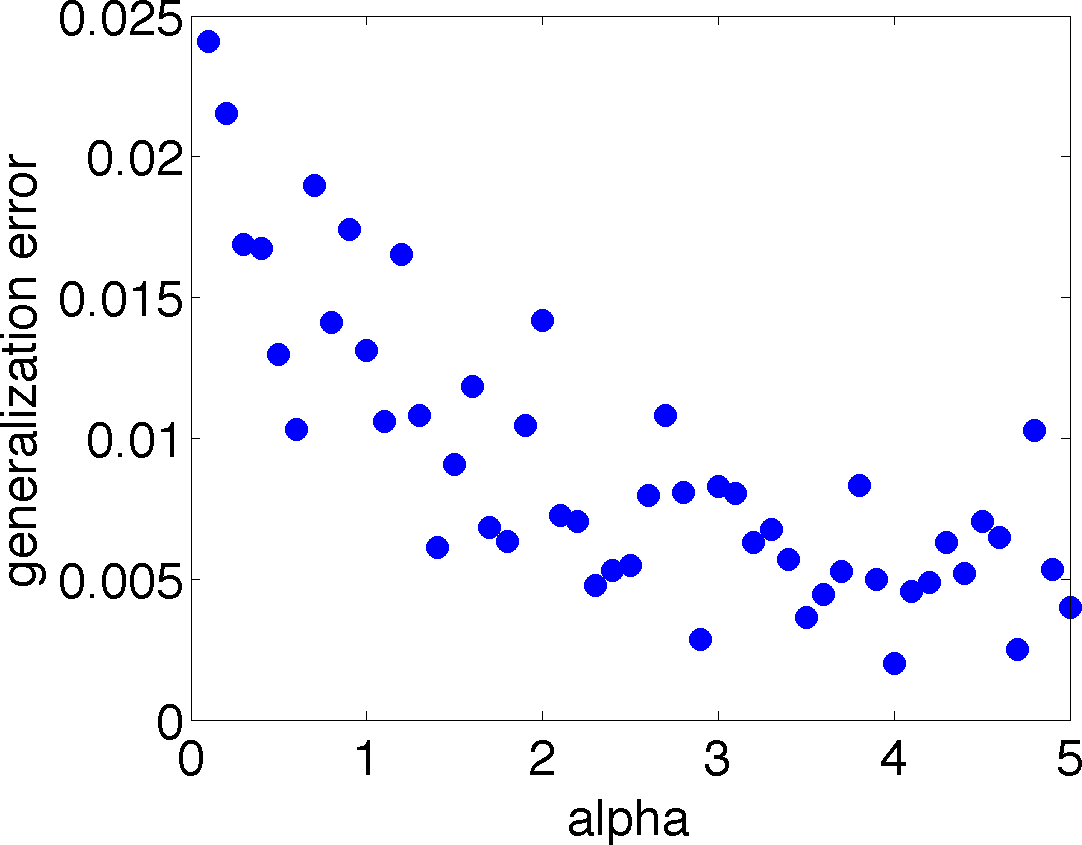
\includegraphics[width=0.9\columnwidth]{./img/finalgeneralizationerrors}
	\caption{Generalization error at the final step of training, for $\alpha = 0.25, 0.5, \dotsc, 5$, $\varepsilon = 0.0005$, $n_{max} = 500$ and $N = 10$.}
	\label{fig:exp:finalgeneralizationError}
\end{figure}

\Cref{fig:exp:finalgeneralizationError} shows the final generalization error for different values of $\alpha$ as an average of $n_d = 10$ iterations with each $\alpha$. We consider a generalization error final when it has converged or when $t_{max}$ has been reached. 

Based on \cref{fig:exp:finalgeneralizationError} we can state that in general the generalization error decreases as $\alpha$ increases. A small $\alpha$ results in a smaller number of patterns, this means that it is more probable that the teacher is not the optimal solution, because of this the generalization error is likely to be larger than with a large $\alpha$ which results in a larger number of patterns and less possible solutions, thus meaning a higher probability the teacher lies near (or is) the solution with maximum stability.

The fluctuations in the $\epsilon_g$ in \cref{fig:exp:finalgeneralizationError} may be due to the random data sets.\\

\Cref{fig:exp:learningcurve} shows the learning curves for different values of $\alpha$ for one dataset per $\alpha$. This figure clearly shows that for smaller values of $\alpha$ the algorithm needed less steps to converge. Furthermore for nearly all values of $\alpha$ the generalization decreased strongly before decreasingly oscillating around its final generalization error. The curves also show that the error can increase. This is because the found solution at that point in time maybe close to the teacher, but still can increase in stability, thus the final solution may lay further away from the teacher (resulting in a higher error). 

One possible explanation for these oscillations is that the optimal weights cannot be formulated as a linear combination of the support vectors. In this case the algorithm continues to add and subtract vectors from the weights, resulting in a constantly changing generalization error. Since our convergence criterion is the stabilization of the generalization error for $P$ steps, these oscillations prevent convergence. 

\begin{figure}
	\centering
	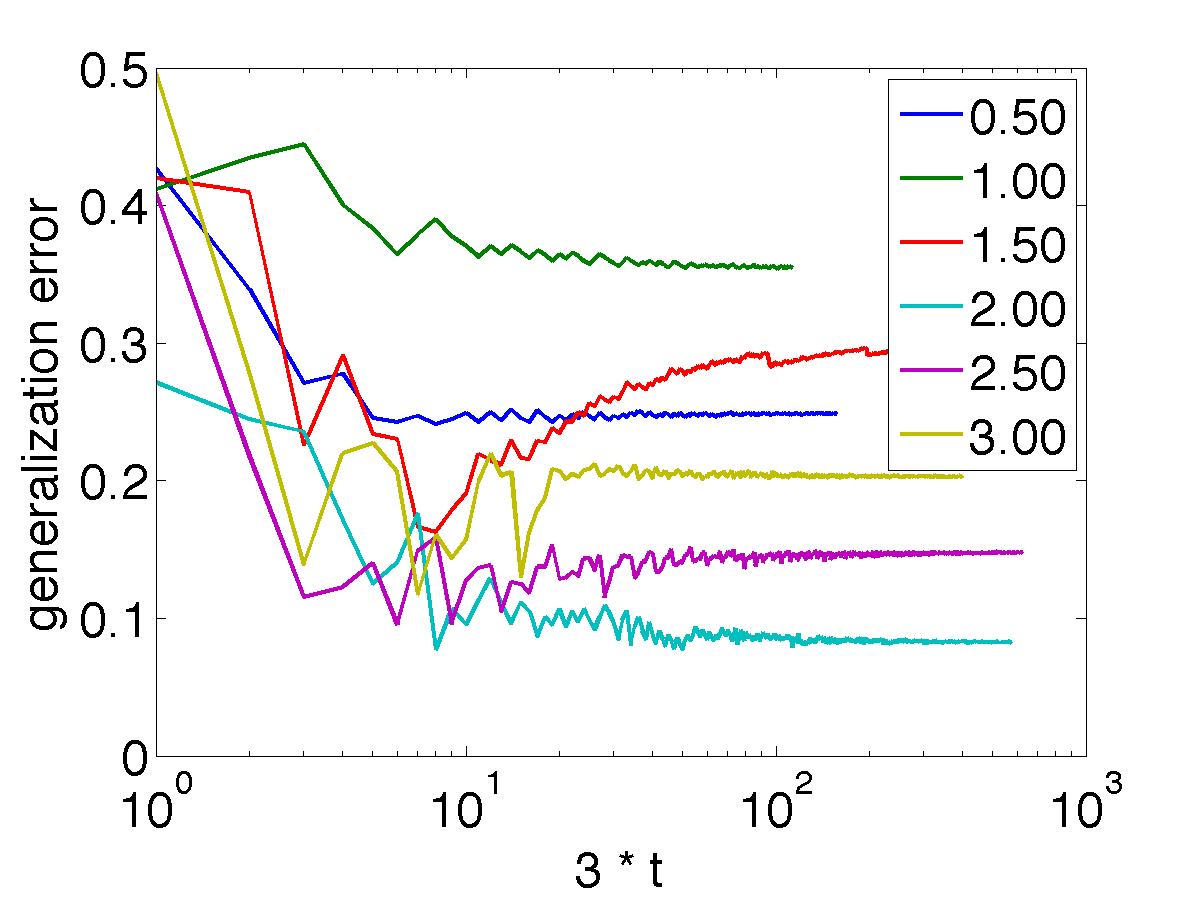
\includegraphics[width=0.9\columnwidth]{./img/N5NMAX500error3}
	\caption{Learning curve for different $\alpha$ for $N = 5$, and $\varepsilon = 0.0005$ and $n_{max} = 500$.}
	\label{fig:exp:learningcurve}
\end{figure}

Smaller datasets converge faster due to the fact that they have less support vectors and thus have fewer factors to consider when computing the optimal weights. 